\section{Product Page}
This section contains the usability analysis of a product page of the website.

\subsection{Informative Axes}
The product page is considered to be an internal page. There the user is "after" the homepage,
but it is not possible to assume that he already knows everything regarding the 6w; 
in fact browsers may take him directly to an internal page (through deep linking). 
So there is the need to replicate at least the most important axes.

\begin{figure}[H]
	\centering
	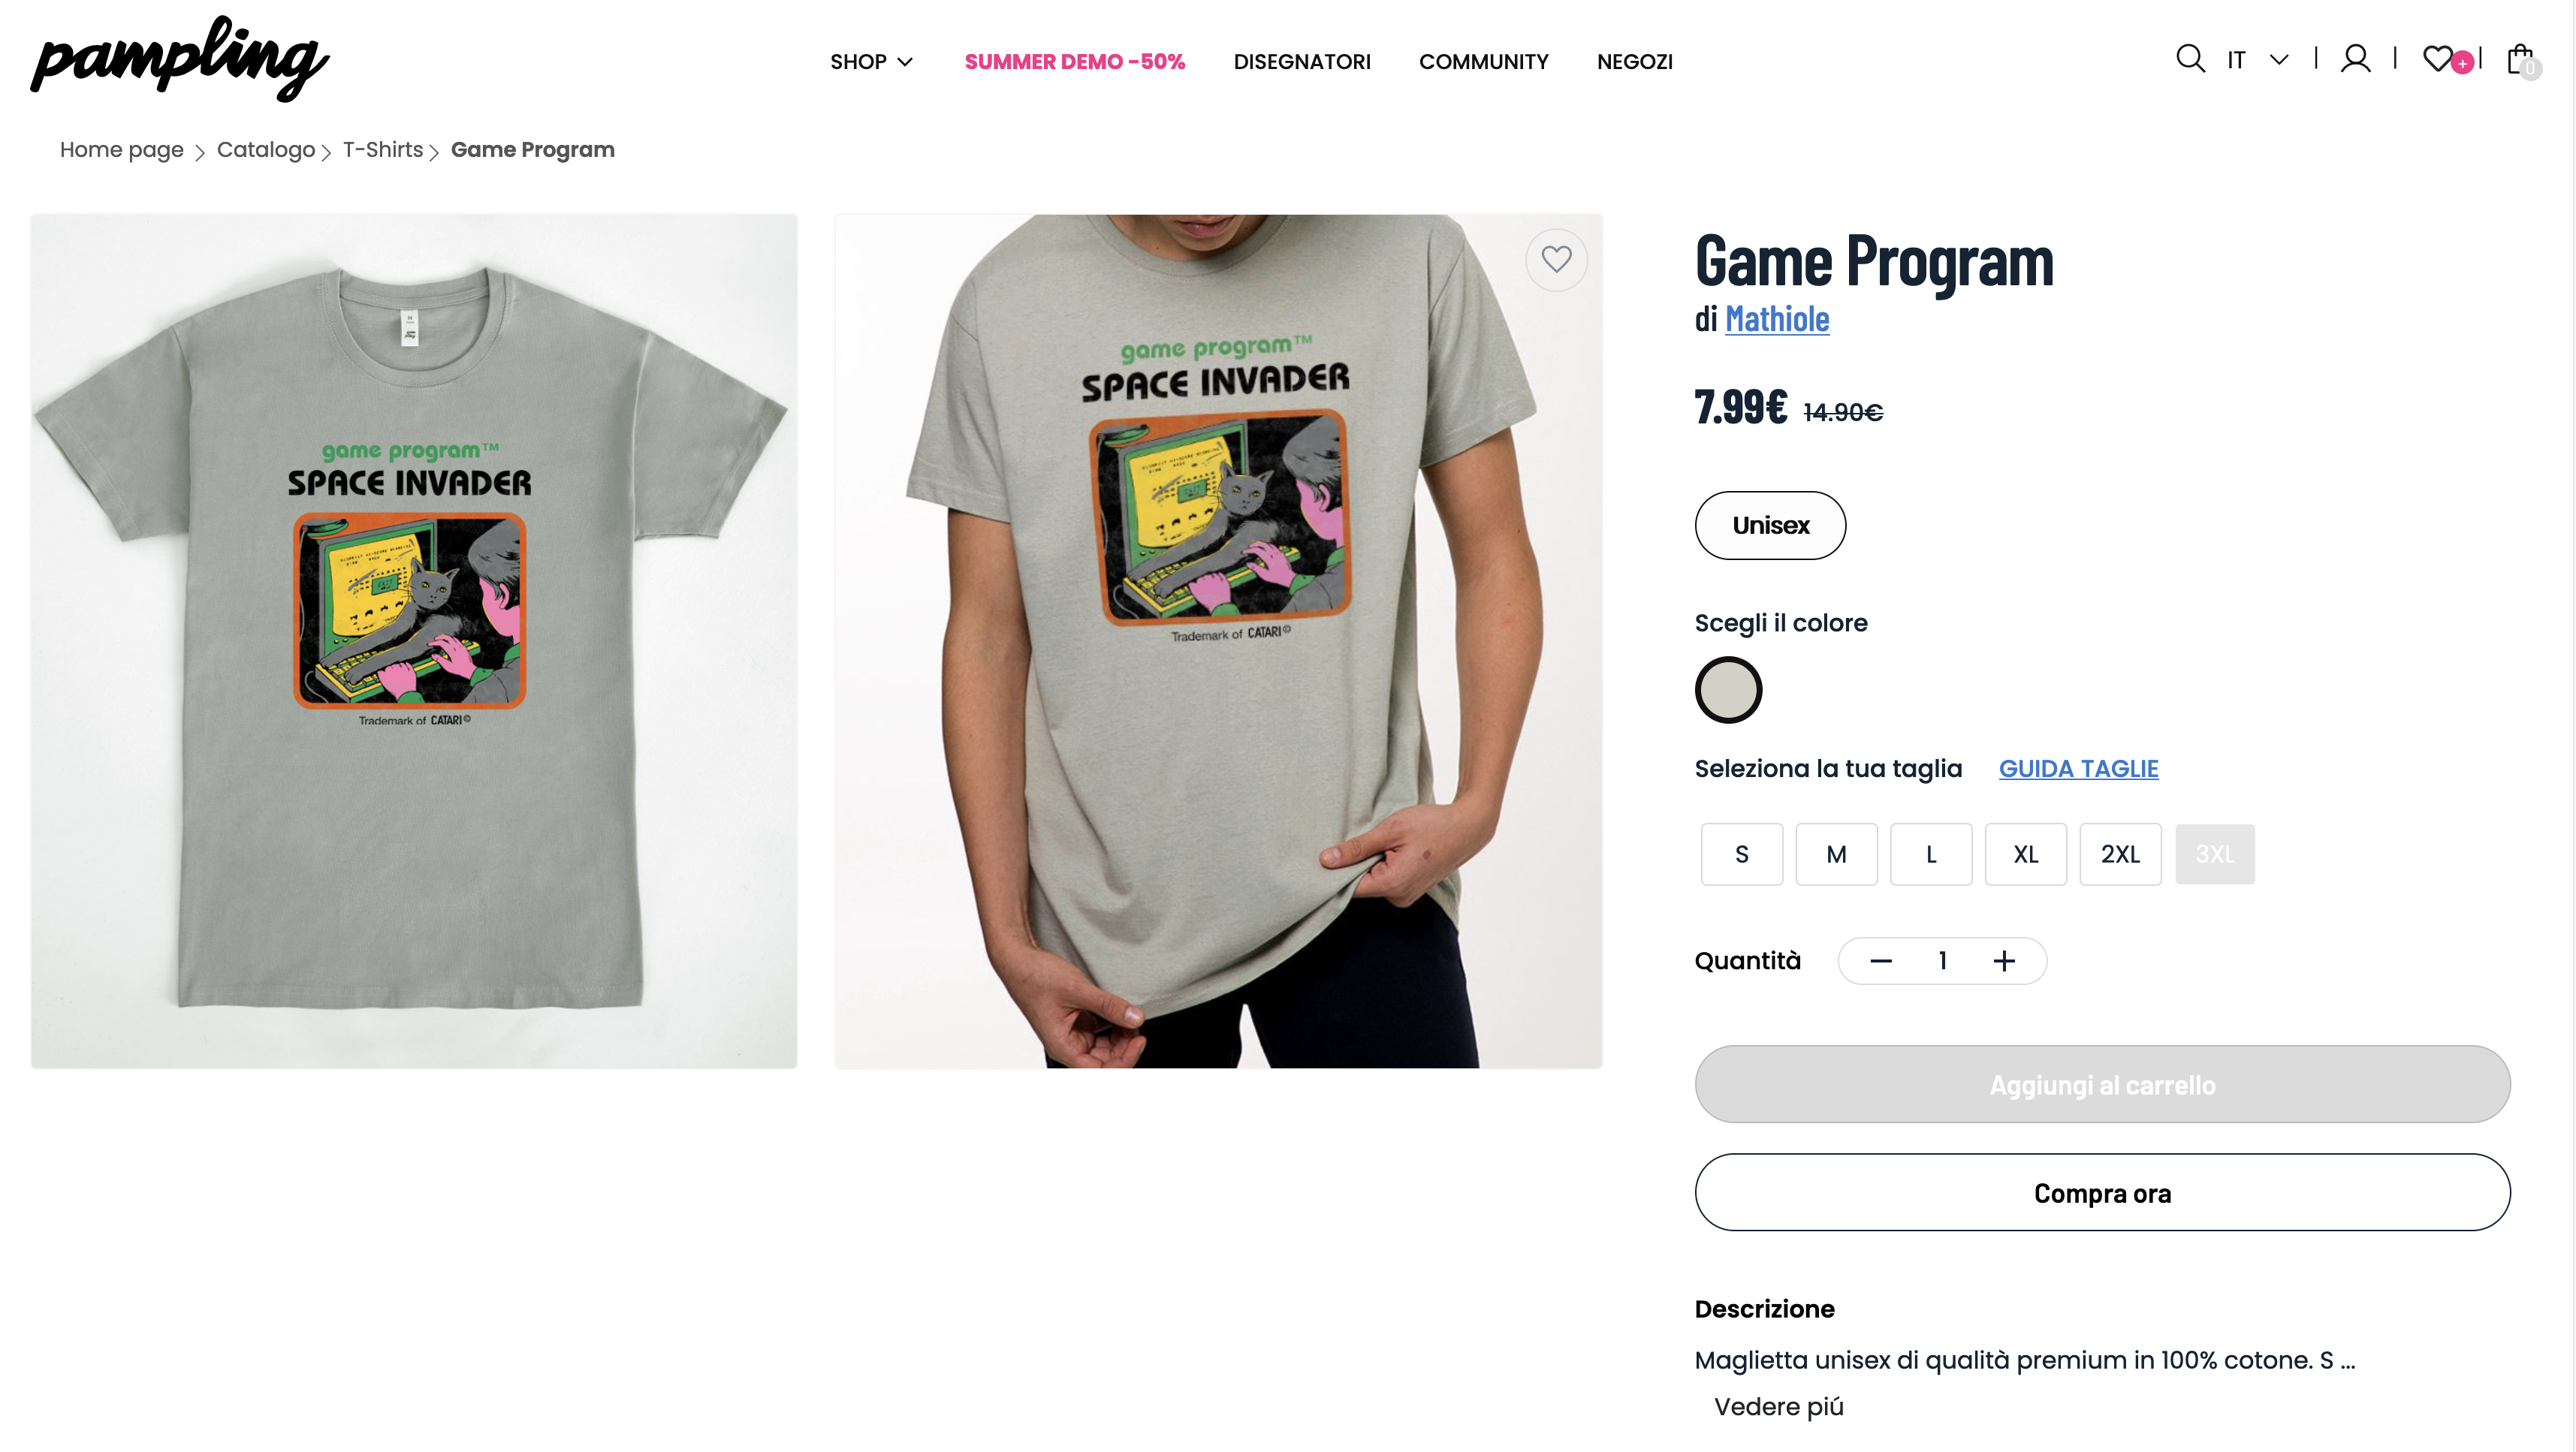
\includegraphics[scale=0.225]{images/product-page.png}
	\caption{product page.}
	\label{fig:product-page}
\end{figure}

\subsubsection{WHERE did the user arrive?}
Even in internal pages it is important for the website to give to the user all the information regarding their relative position withinin the website. \\

In the product page shown in \cref{fig:product-page}, the breadcrumbs are present and give the absolute path 
from the homepage. In this way users always know where they are and they don't get lost inside the website. 

\subsubsection{WHO is behind the website?} 
The "who" axis should give the information about the website's owner.\\

The logo in the top left corner is still present, which is good to immediatly identify the owner of the website.
Since there's not any slogan together with the logo, the user will be able to actually identify the company only
if they already know it. For new users coming directly from search engine and that don't already know it, no
further information is given for them to trust the page.


\subsubsection{WHY should the user stay?} 
The "why" axis should provide motivations to users to persuade them to stay and navigate within the website.\\

All the main information regarding the product are visible without the need
of scrolling, like for example the price, the available choices for the size
and type and the quantity to purchase. This is good because the users will immediatly understand if 
the page contains what they're looking for.


\subsubsection{WHAT choices does the user have?} 
Another important axis is the "what" one. It should give the users access to all the possible destinations of the website.\\

The menu at the top is still present, that' the correct choice.

\subsubsection{WHEN (latest news)} 
This axis should provide to the users all the latest news regarding the products and the company.\\

By scrolling a little down, the most recent reviews from other users can be found, which are a little
indicator of the activity of the website. Also, when some special offers are acrive, in the top menu
the "special" voice chages indicating the current active offer. For example, in \cref{fig:product-page}, 
the "Summer Demo -50\%" is active. This also gives an indicator of activity and novelty to the users.

\subsubsection{HOW to arrive where the user wants?} 
The axis should offer tools to the users in order to let them access and collect information in a smart way.\\

Again, the menu and the search bar are available to the users, permitting them to reach every part of the 
website exactly as they were in the homepage.

\subsection{F-shape Map}
As said before, the most important components of the webpage should be placed within the top center of the webpage. \\
Since the general layout of the page is still the same as the one of the homepage, the F-shape map
is respected. 
The only difference from the homepage is that now the content is divided into two different column: 
the one on the left containing the images of the product while on the right there are the product's information.

This is a typical structure for the product page so, even if the important information about the product 
are on the right side of the page, the user will notice them.

\subsection{Product}
The product page should contain the following components:
\begin{itemize}
	\item Product’s visual description;
	\item Product’s textual description;
	\item Price;
	\item Add to cart button;
\end{itemize}

\subsubsection{Visual Description}
Images in this kind of e-commerce are fundamental for the user to know what the product is and 
its main features.
At least two images are always present showing the design printed on the product and/or the final 
product itself. All the images are clickable and can be zoomed in. This is particularly good
since users tend to click on them. 
If the images are more than two, the third one remains half hidden and some scroll or a click on it
is required to see it entirely.

\subsubsection{Textual Description}
The textual description of the product is visible only in its first line since the others are hidden 
behind a "See all" button. 
It contains a description of the material, the features and the techiniques
to take care of the product. 
There is also a "Get it FOR FREE" section that shows up only if the "See all" button is clicked and after
doing a little scroll down that informs about a kind of "fidelity" offer.
The fact that these information are hidden is not good since the users will probably not read them,
unless they are really inerested in the product. In particular the "Get it FOR FREE" section that 
might be really interesting for the users and might also bring them into the community.
The need of scrolling also is not good since the users in general al not willing to scroll down, 
unless again are really interested in the product.
Other important (but not complete) information about the return policy and the delivery become visible
only after scrolling down and clicking on their cards. Again, not a good design since they don't even
seem clickable in the first place. 


\subsubsection{Price}
The price is visible and well highlighted in the top of the product page. 
It does not contain the cost of the delivery, that is not mentioned anywhere inside the product page.
Only during the checkout, the additional cost for the shipping can be calculated as shown in \cref{fig:checkout-1}.
Also, an information about a threshold for a free delivery is shown now: this information would 
be better to be given before arriving to the checkout. 
\begin{figure}[H]
	\centering
	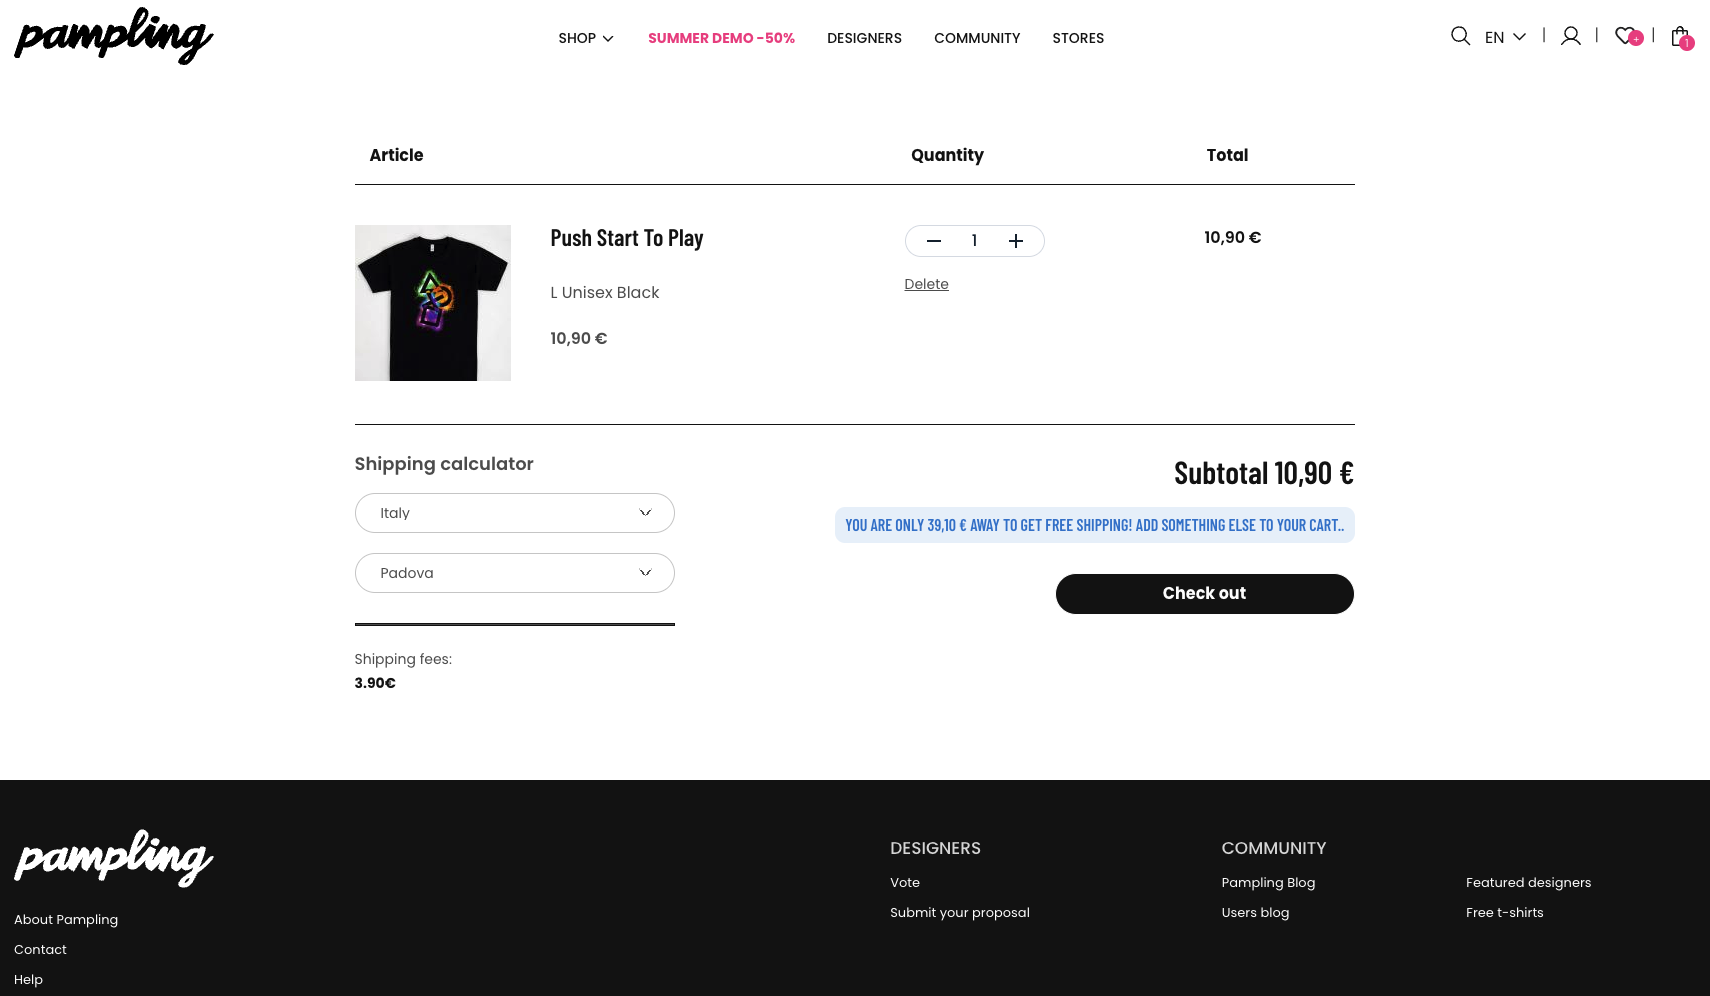
\includegraphics[scale=0.225]{images/checkout1.png}
	\caption{before checkout.}
	\label{fig:checkout-1}
\end{figure}


\subsubsection{Checkout}
During the checkout procedure, the users are given the possibility to log-in or proceeding as
guests, as shown in \cref{fig:checkout-2}. The fact that users are given the choice to not register
to the website is good, since sometimes they might not have time for that. Still, users are informed 
of the advantages of creating an account. 
After that, for both logged-in and guest users, the information about the delivery are required.
Pick-up points may be chosen for the delivery, a service that users appreciate.
Once inserted an address, the final price inclusing also the delivery costs is shown on the right side
of the page, together with all the products in the shopping chart and their characteristics.
This is good since it will give users a final sum up of their purchase and the possibility to check for that the 
correctness of the products that they're going to buy. 

\begin{figure}[H]
	\centering
	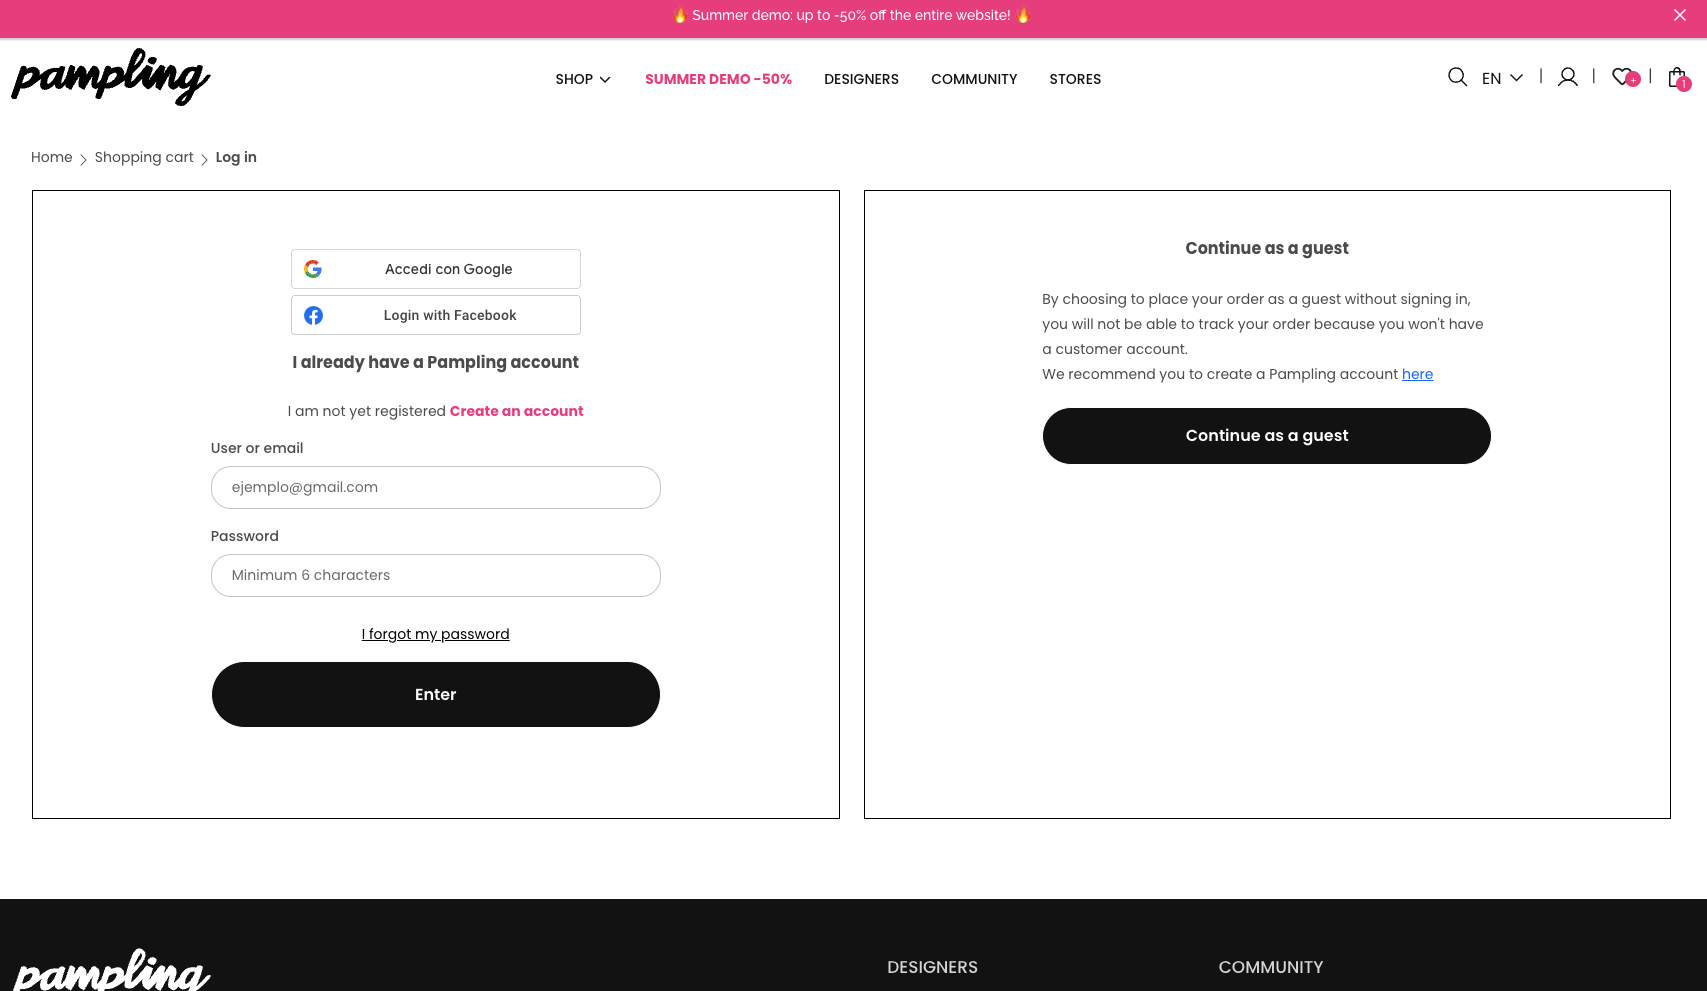
\includegraphics[scale=0.225]{images/checkout2.png}
	\caption{checkout.}
	\label{fig:checkout-2}
\end{figure}
\begin{figure}[H]
	\centering
	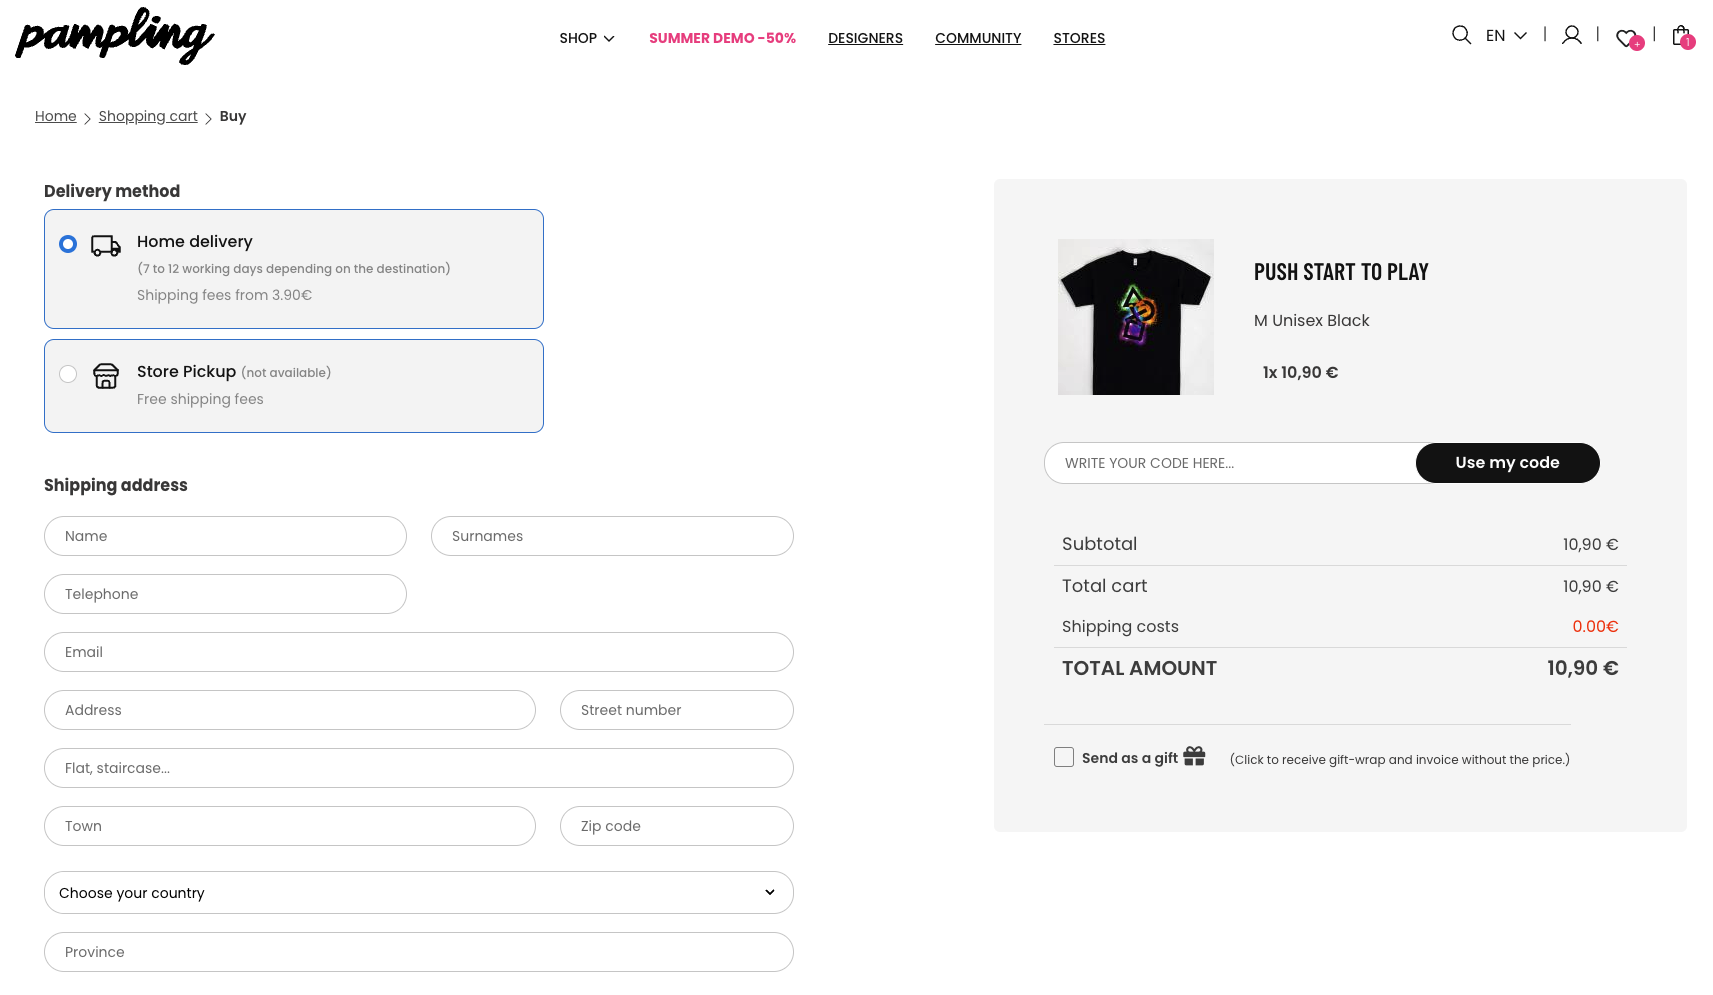
\includegraphics[scale=0.225]{images/checkout3.png}
	\caption{checkout.}
	\label{fig:checkout-2}
\end{figure}

